\subsection{L'interface solide/liquide/gaz et angle de contact} \todo{Lecture 4}

On definit $\gamma _{\mathrm{sl}},\gamma _{\mathrm{sg}}$ et $\gamma _{\mathrm{lg}}$ qui denotent respectivement la tension superficielle pour l'interface solide/liquide, solide/gaz et liquide gaz. En equilibre la somme des forces sur la ligne triple de contact entre les trois phases est nulle. On a selon $\boldsymbol{e}_{x}$ que $\boldsymbol{F}\propto\gamma$ . En particulier on a:
\begin{theorem}[Loi de Young]
$$
\cos \theta=\frac{\gamma _{\mathrm{sg}}-\gamma _{\mathrm{sl}}}{\gamma _{\mathrm{lg}}}
$$
ou $\theta$ est l'angle de contact.
\begin{itemize}
\item $0<\gamma _{\mathrm{sg}}-\gamma _{\mathrm{sl}}<\gamma _{\mathrm{lg}}\Rightarrow0<\cos \theta<1\Rightarrow0<\theta<90$ et on dit qui il y a un "bon mouillage".
\item $\gamma _{\mathrm{sg}}-\gamma _{\mathrm{sl}}>\gamma _{\mathrm{lg}}\Rightarrow$"$\cos \theta>1$" et on a une "mouillage totale".
\item $-\gamma _{\mathrm{lg}}<\gamma _{\mathrm{sg}}-\gamma _{\mathrm{sl}}<0\Rightarrow-1<\cos \theta<0\Rightarrow90<\theta<180$ et on a un "mauvais mouillage".
\item $\gamma _{\mathrm{sg}}-\gamma _{\mathrm{sl}}\leq\gamma _{\mathrm{lg}}\Rightarrow$ "$\cos \theta<-1$" et on une super-hydrophobie, un "effet Lotus".
\end{itemize}
\end{theorem}
\subsection{Loi de Laplace}
A l'interieur d'un ballon, il y a une surpression.
\begin{question}
Et a l'interieur d'une goutte d'eau ou d'une goutte de savon?
\end{question}
\begin{answer}
On regarde une goutte liquide spherique en apesanteur.
\begin{figure}[h!]
\centering
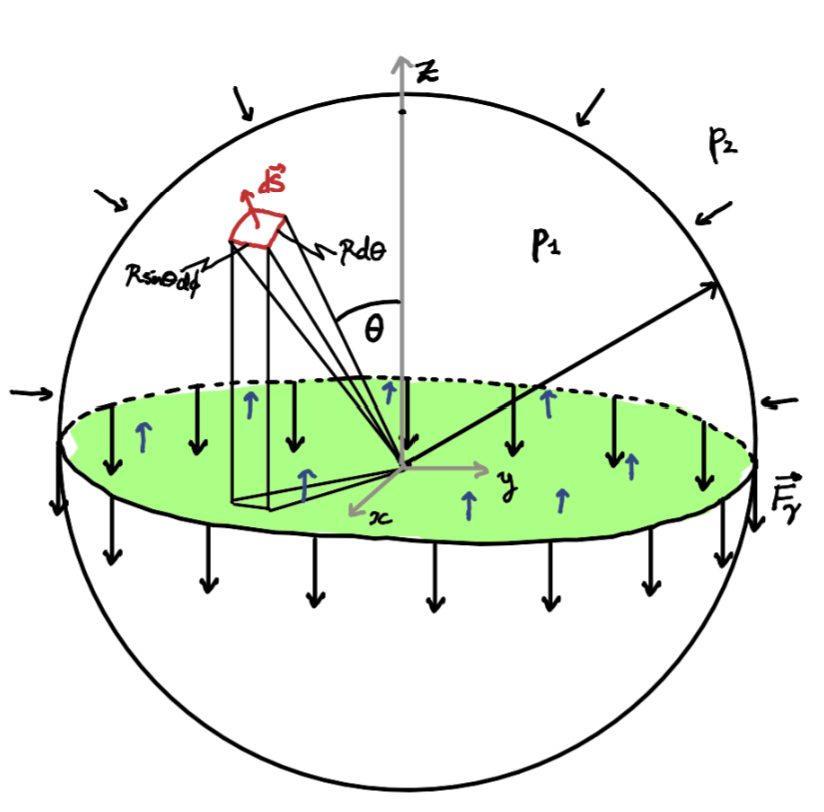
\includegraphics{goutte}
\end{figure}
ou $d\boldsymbol{S}=R~d\theta \cdot R\sin \theta ~d\phi~\boldsymbol{e}_{r}$. Sur la demi-sphere on a les forces $\boldsymbol{F}_{\gamma}=-2\pi R\gamma~\boldsymbol{e}_{z}$,$\boldsymbol{F}_{p_{1}}=\pi R^{2}p_{1}~\boldsymbol{e}_{z}$ et $$\boldsymbol{F}_{p_{2}}=\iint _{S}-p_{2}~d\boldsymbol{S}=\int_{0}^{2pi}\int_{0}^{\pi /2} -p_{2}~\boldsymbol{e}_{r}\cdot R^{2}\sin \theta~d\theta~d\phi$$
comme $\boldsymbol{e}_{r}=(\sin \theta \cos \phi,\sin \theta \sin \phi,\cos \theta)$ alors car par symetrie les composantes selon $x$ et $y$ sont nulles:
\begin{align*}
\boldsymbol{F}_{p_{2}} & =\boldsymbol{e}_{z}~\int_{0}^{2\pi} \int_{0}^{\pi/2} -p_{2}R^{2}\sin \theta \cos \theta \, d\theta  \, d\phi \\
 & =\boldsymbol{e}_{z}(-p_{2}R^{2})2\pi\left[ \frac{1}{2}\sin ^{2}\theta \right]^{\pi/2}_{0} \\
 & =-\pi R^{2}p_{2}~\boldsymbol{e}_{z} 
\end{align*} 

Donc
$$
\sum \boldsymbol{F}^{\mathrm{ext}}=-2\pi R\gamma~\boldsymbol{e}_{z}+\pi R^{2}p_{1}~\boldsymbol{e}_{z}-\pi R^{2}p_{2}~\boldsymbol{e}_{z}=0
$$
donc dans une surface spherique on defini la Loi de Laplace
$$
p_{1}-p_{2}=\frac{2\gamma}{R}
$$
\end{answer}
\begin{theorem}[Loi de Laplace]
Pour rayons de courbures principales $R_{1}$ et $R_{2}$ au point $M$ de la surface $S$:
$$
p_{1}=p_{2}+\gamma\left( \frac{1}{R_{1}}+\frac{1}{R_{2}} \right)
$$
Cas a connaitre:
\begin{itemize}
\item Sphere: $R_{1}=R_{2}=R$
\item Cylindre : $R_{1}=R$ et $R_{2}=\infty$
\item Plan : $R_{1}=R_{2}=\infty$
\end{itemize}
\end{theorem}